The \gls{MSFR} is a reference fast-spectrum \gls{MSR} concept developed
under the \gls{EVOL} and \gls{SAMOFAR} projects. The main reactor
specifications and schematic view are shown in Table \ref{table:msfr} and
Figure \ref{fig:msfr}, respectively. Developed from the \gls{MSBR}, the
\gls{MSFR} is intended to run primarily on a closed thorium fuel cycle with
continuous online fuel reprocessing. Several reasons motivated the omission of
graphite moderators from the \gls{MSFR} design. Graphite is susceptible to
long-term radiation damage and replacement is likely to be necessary during
the operating lifetime of the reactor. Graphite also has a positive
temperature coefficient of reactivity; eliminating graphite from the design
ensures a greater safety margin \cite{mathieu_thorium_2006}. While negative
temperature coefficients are attainable with very thermalized spectra,
breeding ratios deteriorated significantly due to parasitic absorption in the
large volume of graphite needed for thermalization
\cite{mathieu_thorium_2006}.
%
\begin{figure}[htb!] 
	\centering
	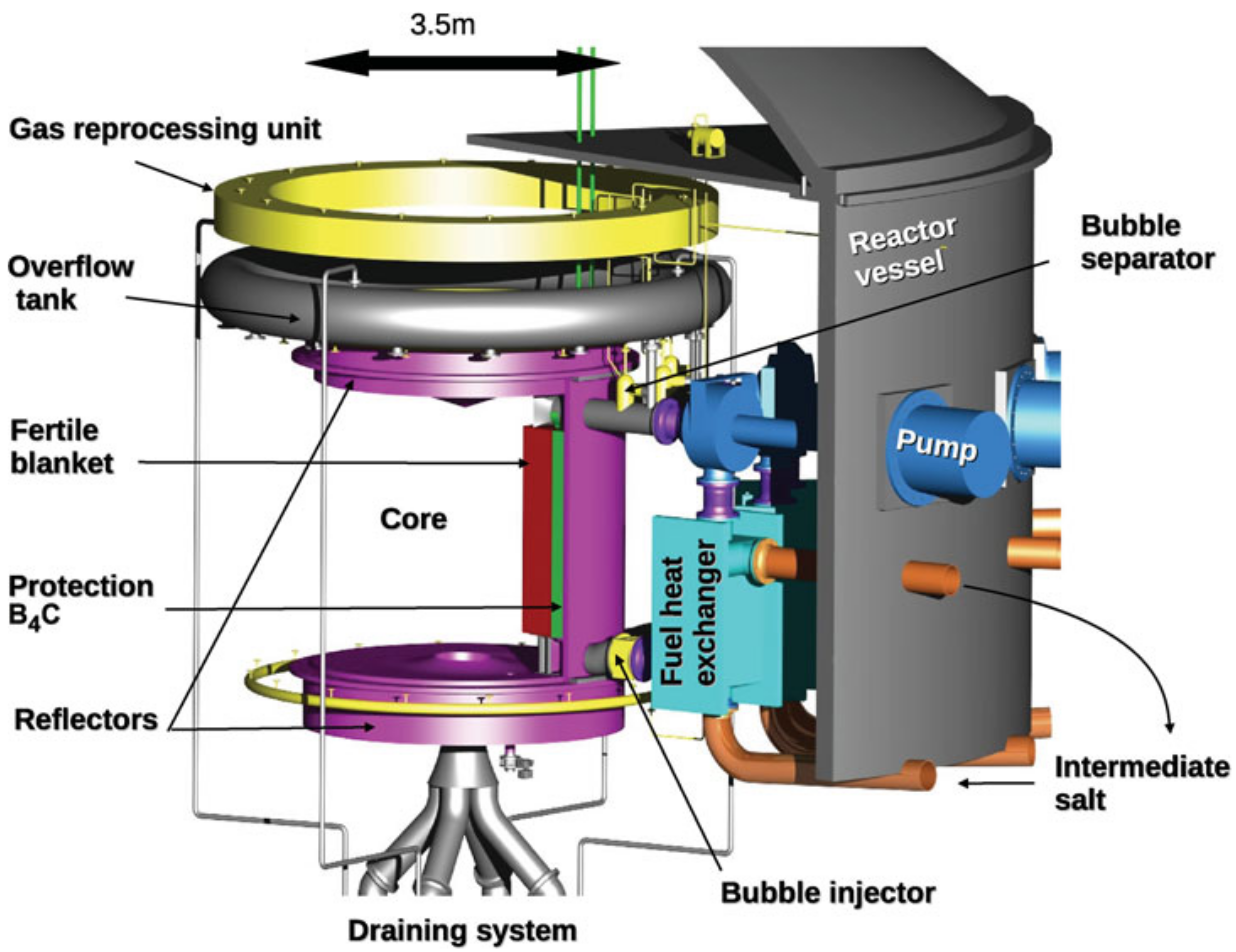
\includegraphics[width=0.6\textwidth]{MSFR}
	\caption{Schematic view of the MSFR concept \cite{serp_molten_2014}.}
	\label{fig:msfr}
\end{figure}
%
\begin{table}[htb!]
    \small
	\caption{Main specifications of the \gls{MSFR} concept
				\cite{serp_molten_2014}.}
	\centering
	\begin{tabular}{ l r }
		\hline
		Parameter & Value \\
		\hline
		Thermal/Electric output [MW$_{\text{th}}$/MW$_{\text{e}}$] & 3000 /
		1500 
		\\
		Salt volume [m$^3$] & 18 \\
		Salt fraction in core & 0.5 \\
		Number of circulation loops & 16 \\
		Nominal flow rate [kg s$^{-1}$] & 18500  \\
		Nominal circulation time [s] & 4.0 \\
		Inlet/outlet temperature [K] & 923 / 1023 \\
		Blanket volume [m$^3$] & 7.3\\
		\hline
	\end{tabular}
	\label{table:msfr}
\end{table}

In the \gls{MSFR} design, fuel salt flows upwards through a 9 m$^3$ central
core region. At the top of the core, the flow separates into sixteen smaller
external loops, each of which passes through a heat exchanger before being
pumped back into the bottom of the core. Other instrumentation are situated
along the external loop for online salt reprocessing and gas sparging. The
core is surrounded axially by nickel alloy reflectors, and radially by a
toroidal blanket tank containing fertile salt for breeding. There is a layer
of boron carbide behind the blanket tanks to protect the peripheral equipment
from excessive neutron damage. In case of severe accidents, there is an
actively cooled freeze plug at the bottom of the core that melts when
temperatures exceed a certain threshold. The fuel salt would drain into a
containment vessel designed to keep it subcritical. Reactivity control under
normal operating conditions is performed by varying pump speeds to take
advantage of the strong thermal feedback. Coupled with the fact that there is
no excess reactivity reserve due to online fuel reprocessing, there are no
control rods in the \gls{MSFR} design.

Although the \gls{MSFR} is primarily designed to operate on the thorium fuel
cycle, it can support a range of start-up fuel and feed compositions. This
versatility is particularly important for the first few \glspl{MSFR} to be
deployed due to the lack of $^{233}$U reserves required for the initial core
loading. In general, the fuel and blanket salts are approximately composed of
eutectic mixtures of 77.5\% LiF - 22.5\% AcF$_4$, where AcF$_4$ represents
actinide fluorides such as uranium, thorium, plutonium, and other \gls{TRU}
fluorides. For an initial composition consisting of $^{232}$Th and $^{233}$U,
the benchmark value for the amount of uranium for criticality under
normal operating conditions is 2.515 mol\%. However, most code verification
studies adjust the ratio of $^{232}$Th to $^{233}$U to achieve exact
criticality at a uniform temperature of 973 K; this ensures that subsequent
neutronics and safety analyses are not affected by the difference in
k$_{\text{eff}}$ values. We performed the same exercise in this thesis.

Power output of the \gls{MSFR} is rated at 3000 MW$_{\text{th}}$ and 1500
MW$_{\text{e}}$. It has a high thermal efficiency due to the high operating
temperature. \glspl{MSR} in general are not restricted by the same pressure
constraints seen in \glspl{LWR}. The inlet and outlet temperature
specifications of the fuel salt are 923 K and 1023 K, respectively. This was
motivated by the need for a minimum 50 K temperature buffer between the
operating temperatures and the melting point of the salt. The \gls{MSFR} has
heat exchangers and an intermediate coolant loop to isolate the power
conversion system from the highly radioactive fuel salt. This also serves as
a layer of containment between the radioactive material and the outside
environment. The exact composition of the intermediate coolant is still under
active study and not finalized yet.

\section{Model Geometry}

For this work, we used a model similar to the reference square-cylindrical
\gls{MSFR} design to benchmark our results against results published by
Fiorina et al. and Aufiero et al. The reference design is a 2-D axisymmetric
model with the sixteen individual external loops homogenized into a single
outer loop as shown in Figure \ref{fig:msfrgeom}. For the multigroup
cross sections and group constants calculations in Serpent, we extended this
2-D axisymmetric model into a 3-D model by a simple full rotation about the
central axis. The material definitions are the same as those specified in the
reference \gls{MSFR} model. Accordingly, the pump and heat exchanger regions
are assumed to be composed of 100\% fuel salt. While this may not be entirely
accurate, the exact details of the pump and heat exchanger systems are still
under active study, and this external loop region is presumed to be of little
neutronic importance due to its position behind the strong boron carbide
neutron absorber layer.
%
\begin{figure}[t!] 
	\centering
	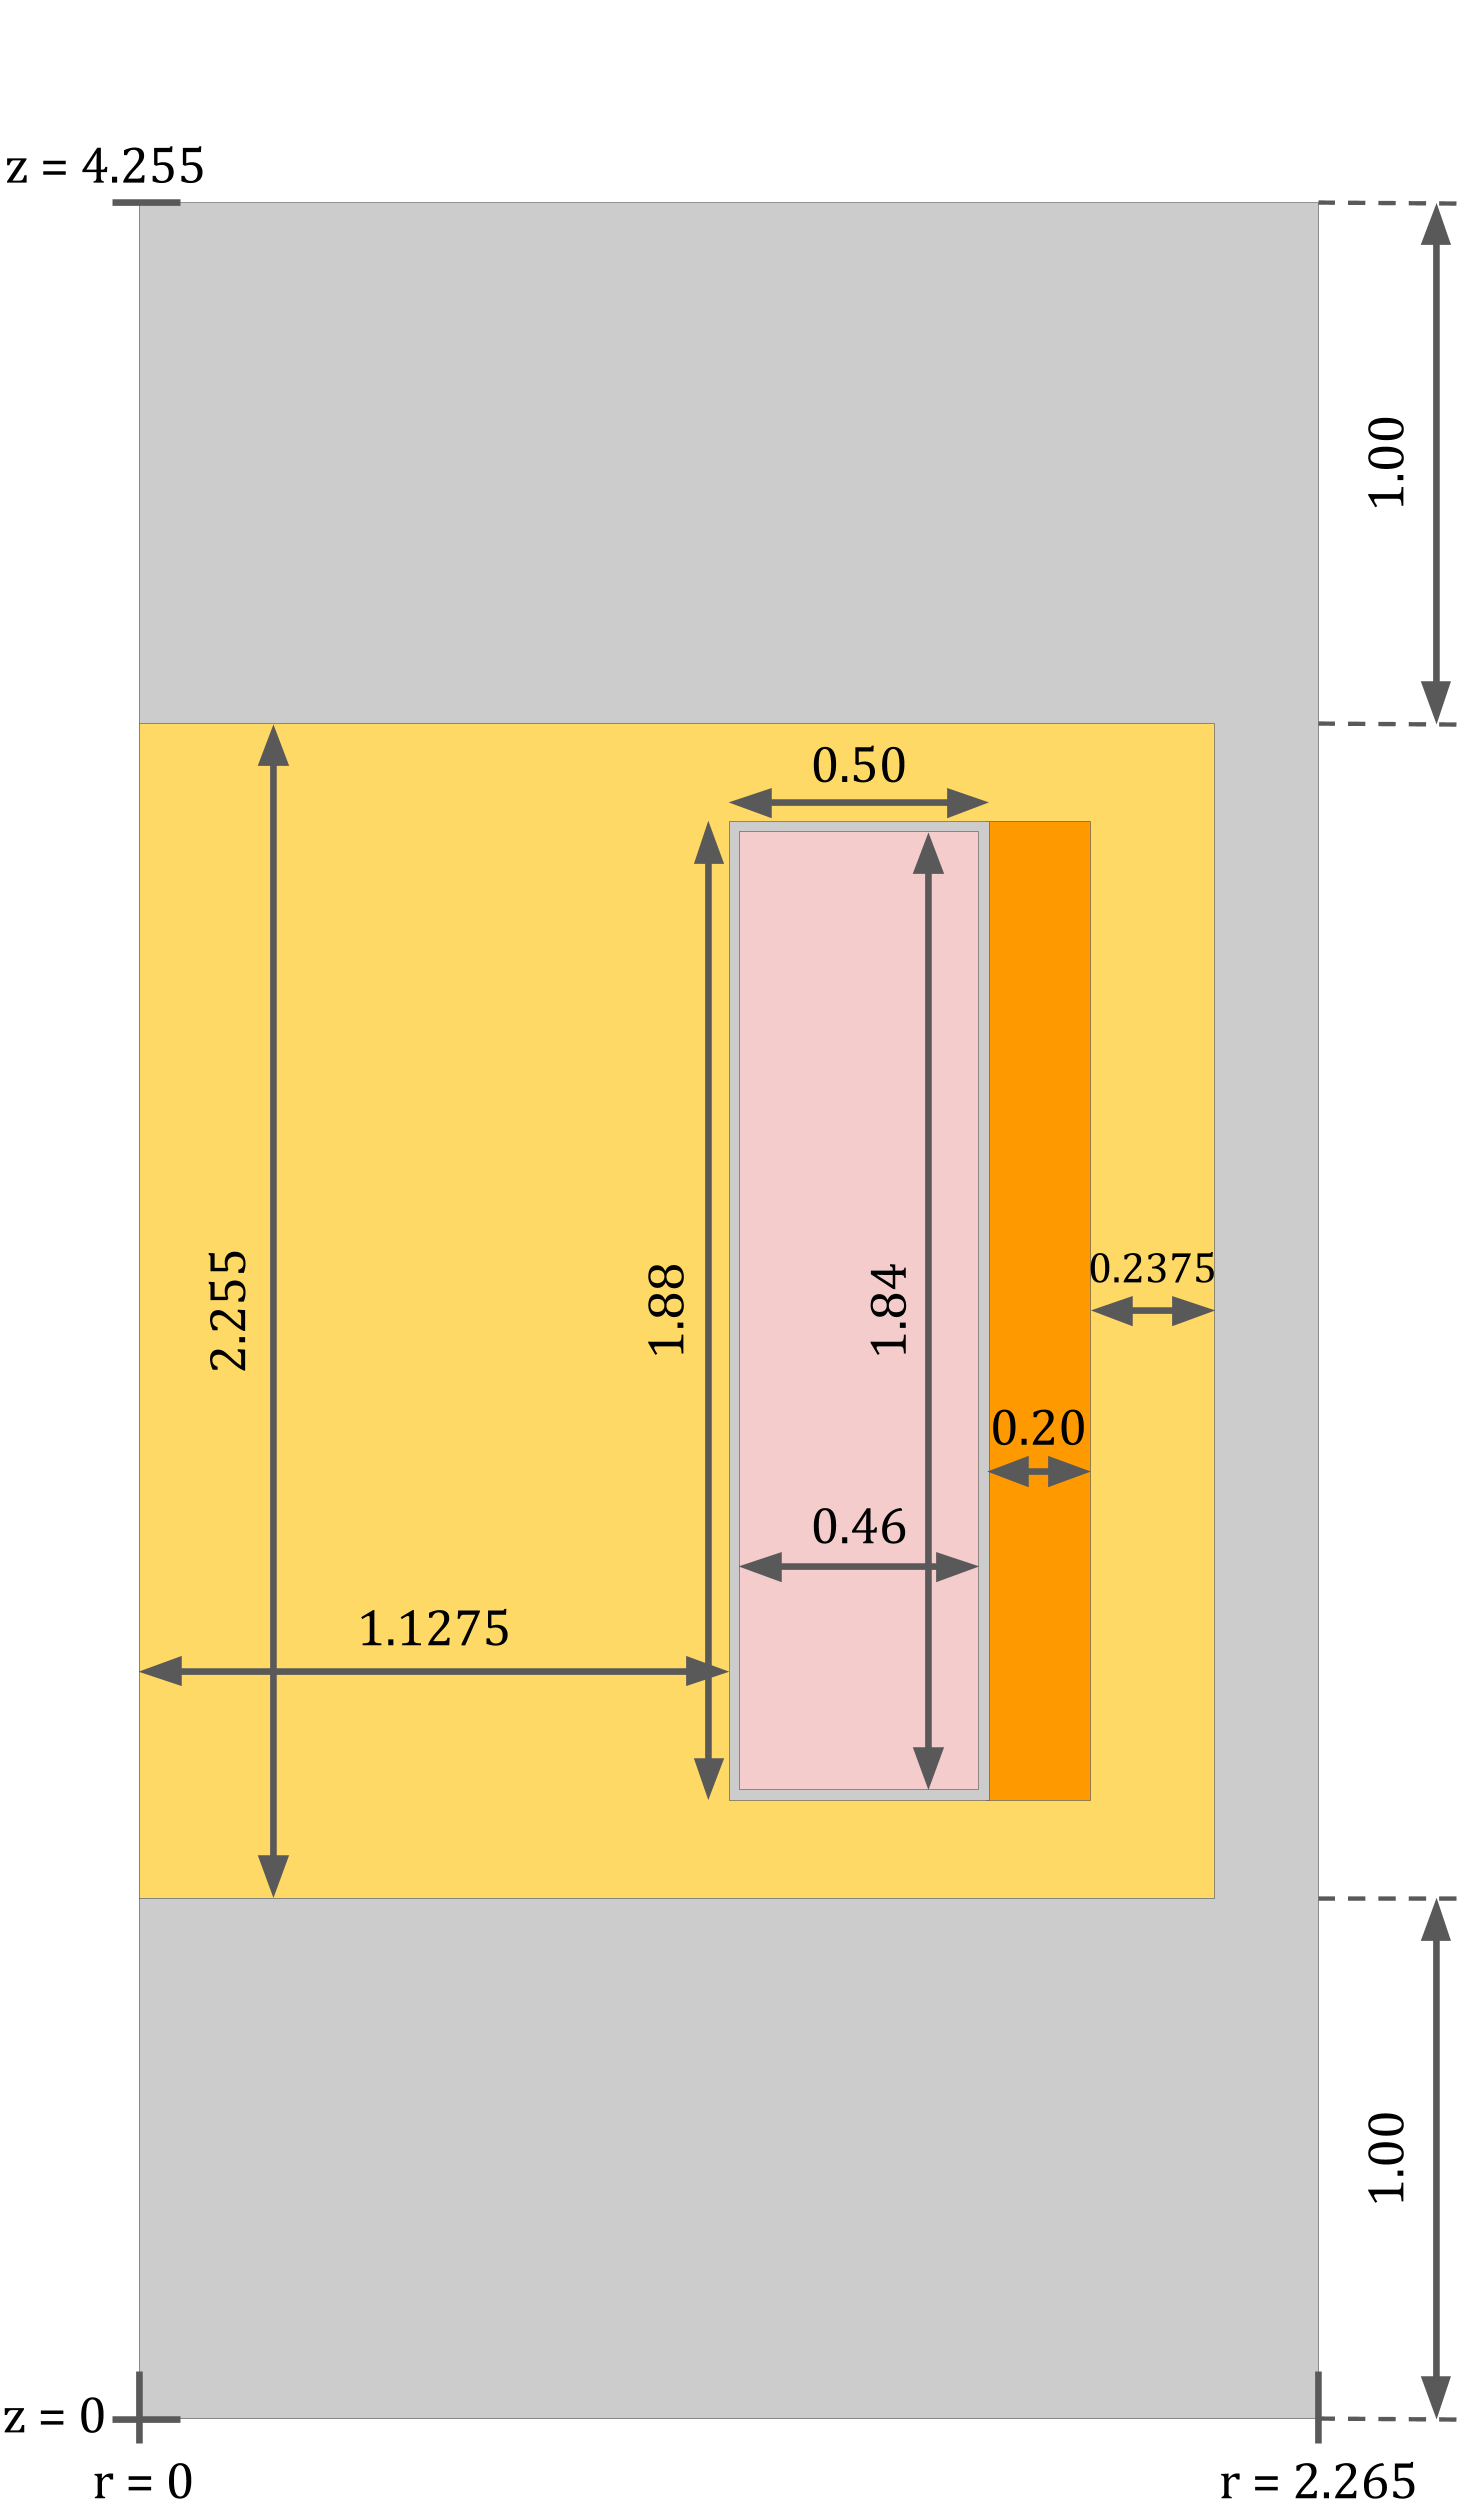
\includegraphics[width=0.5\textwidth]{msfr-geom}
	\caption{2-D axisymmetric model of the \gls{MSFR} core used for the
	simulations in Serpent. All dimensions are in meters.
	\cite{brovchenko_neutronic_2019}}
	\label{fig:msfrgeom}
\end{figure}

Although we used the exact reference model for generating group constant data
from Serpent, there are two minor differences between the \gls{MSFR} model
geometry we used in Moltres, and the Polimi/TUDelft models. The
first difference is a relative
minor change to the mesh by the exclusion of the 2 cm thick structural
material around the blanket tank that separates the fuel and blanket salts.
We removed this feature in our finite element mesh as we encountered
difficulty meshing this layer that is relatively much thinner than the rest of
the model. Any impact on the
neutron flux is expected to be minimal. Furthermore, we solved for the
temperature distribution only in the primary loop and applied homogeneous
Neumann boundary conditions for temperature on the core walls, as was done in
the Polimi/TUDelft models. Therefore, we believe the overall impact on the
results is negligible.

The second difference pertains to the modeling of the external loop. In its
current implementation, Moltres lacks pump- and heat exchanger-equivalents in
the code. Thus, the external loop, beyond the central region of the primary
loop where most of the fissions take place, is modeled as a 1-D pipe with a
point heat sink to represent the heat exchanger. Instead of pumps, the flow is
driven by Dirichlet boundary conditions for velocity on the inlet and outlet
boundaries of the central regions of the primary loop, and the 1-D external
pipe geometry. All flow-dependent variables such as temperature, \glspl{DNP},
and decay heat precursors are fully conserved as they loop around between the
two regions. As a result, this approach shares some similarities with the
geometric multiscale modeling approach by Zanetti et al.
\cite{zanetti_geometric_2015}. Future models could
create a better representation of the primary loop by implementing a whole
continuous loop with pressure increases and drops corresponding to the pumps
and heat exchangers.

\section{Material Specifications}

This section discusses the material specifications of the various reactor
components in the \gls{MSFR}.

\subsection{Molten Salt}

As mentioned before, the fuel and blanket salts are comprised of a 77.5\% LiF
- 22.5\% AcF$_4$ mixture. This is the reference salt composition of the
\gls{MSFR} at start-up. Typically, researchers working with the \gls{MSFR}
model calculate the exact actinide composition by varying the $^{232}$Th to
$^{233}$U ratio to obtain a $k_{\text{eff}}$ value of 1 at a uniform
temperature of 973 K. Thus, the exact actinide compositions vary depending on
the nuclear data library and neutron transport code. The exact composition
used for this work can be found in the Results chapter. We assume that the
effects of these composition variations on the reference physical properties
of the fuel and blanket salt are negligible. Table \ref{table:prip} shows
relevant physical properties of the fuel and blanket salts.
%
\begin{table}[htb!]
\small
\centering
\caption{Properties of the fuel and blanket salts LiF-AcF$_4$.}
\begin{tabular}{l l r r}
\toprule
Property & Formula & {Value at 973 K} & Validity Range\\
\midrule
Melting temperature [K] & 841 & {N/A} & 1 bar \\
Boiling temperature [K] & 1874 & {N/A} & 1 bar \\
Density, $\rho$ [kg m$^{-3}$] & $4094-0.882 \cdot (T-1008)$ & $4125$ & 893-1123 K \\
Dynamic viscosity, $\mu$ [Pa s] & $\rho \cdot 5.55 \times 10^{-8} \cdot e^{3689/T}$ & $1.015$ & 898-1121 K \\
Thermal conductivity, $k$ [W m$^{-1}$ K$^{-1}$] & $0.928+8.397 \times 10^{-5} \cdot T$ & $0.01010$ & 891-1020 K \\
Specific heat, $c_p$ [J kg$^{-1}$ K$^{-1}$] & $-1111+2.78\cdot T$ & $1594$ & 867-907 K \\
\bottomrule
\end{tabular}
\label{table:prip}
\end{table}

\subsection{Structural Materials}

The reflectors on the periphery of the reactor core and the blanket tank are
made of a nickel-based alloy provided from reference specifications
\cite{delpech_reactor_2009}. Table \ref{table:refl} details the compositions
of the nickel-based alloy and boron carbide absorber. The alloy has a density
of 10 g cm$^{-3}$. The material composition of the reflectors may be subject
to minor changes, but it is not a major concern as the reflectors are not
situated in regions of high neutron flux. The \gls{MSFR} also includes a 20 cm
layer of boron carbide (B$_4$C) to protect the heat exchangers and pumps from
neutron irradiation. The reference specifications indicate that natural boron
is used, which is composed of 19.8 \% $^{10}$B and 80.2 \% $^{11}$B, with an
overall density of 2.52 g cm$^{-3}$. 
%
\begin{table}[htb!]
\footnotesize
\centering
\caption{Composition (mol \%) of the nickel-based alloy used in the simulation
of the \gls{MSFR} in this work.}
\begin{tabular}{l l l l l l l l l l l l l}
\toprule
Ni & W & Cr & Mo & Fe & Ti & C & Mn & Si & Al & B & P & S \\
\midrule
79.432 & 9.976 & 8.014 & 0.736 & 0.632 & 0.295 & 0.294 & 0.257 & 0.252 & 0.052 & 0.033 & 0.023 & 0.004 \\
\bottomrule
\end{tabular}
\label{table:refl}
\end{table}
